%\documentclass[letterpaper,11pt]{article}
\documentclass[a4,11pt]{article}
\usepackage{geometry}
\usepackage{xcolor}
\usepackage{amsmath}
\usepackage[some]{background}


\usepackage[
    type={CC},
    modifier={by-nc-sa},
    version={4.0},
]{doclicense}

\usepackage[hypcap=false,font=small,labelfont=bf]{caption} % Required for specifying captions to tables and figures
\usepackage{hyperref}

\newcommand\fnurl[2]{%
    \href{#2}{#1}\footnote{\url{#2}}%
}

\definecolor{titlepagecolor}{cmyk}{1,.60,0,.40}

\DeclareFixedFont{\bigsf}{T1}{phv}{b}{n}{1.5cm}

\backgroundsetup{
    scale=1,
angle=0,
opacity=1,
contents={\begin{tikzpicture}[remember picture,overlay]
    \path [fill=titlepagecolor] (-0.5\paperwidth,5) rectangle (0.5\paperwidth,10);  
\end{tikzpicture}}
}
\makeatletter                       
\def\printauthor{%                  
    {\large \@author}}              
\def\printdate{%
    {\large \@date}}
\makeatother
\author{%
    \textbf{Adam Balawender} \\
    \vspace{2pt}
    \textit{Faculty of Electronics}\\
    \vspace{2pt}
    \textit{Wroclaw University of Science and Technology}\\
    \vspace{40pt}
    Instructor:\\\textit{Witold Paluszynski, Ph.D.}\\
    Class:\\\textit{Intermediate Project}
    }
\date{2018 January}

\begin{document}
\hypersetup{pageanchor=false}
\begin{titlepage}
    \BgThispage
    \newgeometry{left=1cm,right=3cm,bottom=2cm}
    \vspace*{2cm}
    \noindent
    \textcolor{white}{\bigsf UART implementation for PRU-ICSS}
    \vspace*{2.5cm}\par
    \noindent
    \begin{minipage}{0.35\linewidth}
        \begin{flushright}
            \printauthor
        \end{flushright}
    \end{minipage} \hspace{15pt}
    %
    \begin{minipage}{0.02\linewidth}
        \rule{1pt}{175pt}
    \end{minipage} \hspace{-10pt}
    %
    \begin{minipage}[c][9cm][b]{0.6\linewidth}
        \vspace{5pt}
        \begin{abstract} 
            The goal of this project is to use the PRU-ICSS to create a fast ( $>$ 1Mbps ) peripheral serial communication device, entirely in software.
            For the sake of testability, UART has been chosen as the implemented device. Although PRU-ICSS may include a hardware UART peripheral, it is not used in this project.

            Hard real-time capabilities of the PRU were combined with the extended I/O hardware and a carefully optimized critical section.
            As a result, the new peripheral has a theoretical maximum speed limit of 4.347MBaud.
            However, due to clock divisor limitations, the maximum configurable speed is 4.168MBaud.

            The new peripheral has been tested to work reliably up to that speed, which is beyond the reach of the FT232RL, a popular UART interface chip.
            It may be used as a base for implementing more complex protocols, such as CAN.
            This document contains the design considerations and the testing setup.
        \end{abstract}
    \end{minipage}
    \vspace*{\fill}
    \center{\printdate}
    \small\doclicenseThis
\end{titlepage}
\restoregeometry
\hypersetup{pageanchor=true}
\pagenumbering{arabic}

\section{Introduction}
            The goal of this project is to use PRU-ICSS to create a fast ( $>$ 1Mbps ) peripheral serial communication device, entirely in software. PRU is an interesting platform, but there are not many projects involving it. Perhaps this work may improve the situation and become a building block for the next, more complex one.

            UART has been chosen mostly because of its low complexity, allowing to focus on platform-related problems, instead of the protocol caveats. UART can also be easily tested and verified by communicating it with other commonly available, inexpensive UART devices.

\subsection{UART}
Universal Asynchronous Receiver-Transmitter is a hardware device for asynchronous serial communication.
Each character is framed as a start bit, 5-9 data bits, optionally a parity bit and one or more stop bits.
Typically, the idle state is high and the start bit is low, as visible in the figure \ref{fig:standard}.

\begin{figure}[h]
    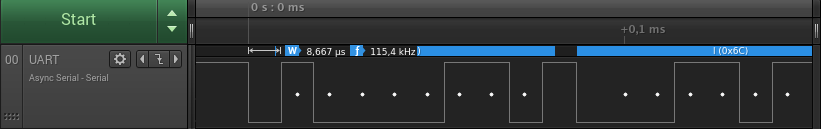
\includegraphics[width=\textwidth]{img/standard.png}
    \caption{Typical UART configuration: 115200 8N1 (115200 Baud, 8-bit of data, no parity, 1 stop bit) }
    \label{fig:standard}
\end{figure}

Communicating UARTs do not share timing system apart from the communication signal, so both devices need to have the same configuration to be able to synchronize and communicate.

\subsection{PRU-ICSS}

The Programmable Real-Time Unit and Industrial Communication Subsystem (PRU-ICSS) consists of two
32-bit RISC cores (PRUs).

The PRUs can be used to implement custom peripheral interfaces, especially in situations where real-time responses are crucial. The PRU cores can be programmed with a small, deterministic instruction set, and can operate independently or in coordination with each other, as well as in coordination with the device-level host CPU\cite{PRU}.

\subsubsection{Hardware details}
Texas Instruments AM335x chip, used to develop this project, is the second-generation PRU (PRUSSv2) with the following specification\cite{TRM}:
\begin{itemize}
    \setlength\itemsep{0em}
    \item 200MHz clock, no pipeline, executing each instruction in a single clock cycle (5ns),
    \item 8KB data and 8KB instruction memories per core, 12KB shared RAM,
    \item enhanced GPIO with the ability of operation in serial or parallel modes,
    \item scratchpad shared by the PRU cores,
    \item multiplier with optional accumulation unit (MAC),
    \item internal peripherals (UART, eCAP, MII\_RT, MDIO, and IEP),
    \item interrupt controller with the possibility of handling and posting events to the host CPU.
\end{itemize}

\subsubsection{Development environment}
Recently, a C/C++ cross-compiler has been developed for the PRUs. The compiler supports C99 and C++03 standards\cite{compiler}. The compiler, as well as GCC toolchain are now a part of the \textit{TI processor SDK}\cite{sdk}.
Example code, as well as setup and compilation instructions can be found in the \textit{pru-software-support-package}\cite{swpkg}. Most of the software provided by TI is licensed as TSPA and is publicly available to use for free.

Drivers to load firmware to the PRUs and control execution are included in the Linux kernel (4.4.91-ti).
Also, a message queue implementation exists to share data between PRUs and the host CPU\cite{rpmsg}.


\section{Design considerations}

 \subsection{Using shift mode for I/O}
 The PRU's extended GPIO modes include shift-in and shift-out. This means that only one pin is used externally to read or output signals, but internally they are visible as 16-bits registers. This is not that important for the transmitter module, but due to oversampling in the receiver (see below), the shift-in mode is crucial in achieving high speed and reliability.

 \subsection{Using separate cores for transmitting and receiving}
 Shift modes only use the first pin of input or output bank, accordingly.
 Also, PRUs have separate pins for input and output.
 However, due to the external pin multiplexer's limitation, the first pin of both banks of a given PRU is the same physical pin, so only one of those will be routed out. Hence the decision to use separate cores.

 \subsection{Using inverted signals}
 The PRU's shift-in input mode has a counter that posts an event every 16 input clock cycles after a 1 is read.
 The UART's standard start bit is 0, so to be able to use the built-in 16-counter, all signals used in this projects are inverted. FT232RL chip can also be programmed to work with inverted signals.

 \subsection{Oversampling in the receiver}
 Due to clock jitter, the receiver needs to read data with a higher frequency. Otherwise, it may happen that some bits will be skipped. Again, due to the 16-counter and 10-bit size of a data unit, this implementation will use 8x oversampling, which means that to receive 1 unit of data, the receiver reads 16 bits, 5 times. Then, it splits every received 16 bits in two groups and does a majority vote. If there are 4 or more \textbf{1}s read among the 8 bit, it understands it as a \textbf{1}.

 \subsection{Clock divisor constraints}
 Shift modes are triggered by the pulses of the internal clock going through two divisors. Each divisor can be set between $1$ and $16$ with the step of $0.5$. This significantly limits the number of available frequencies.

 \section{Results}

 \subsection{Testing setup}
 The testing setup used consists of:
 \begin{enumerate}
     \item BeagleBone Black - a development board based on TI AM335x chip with PRU-ICSS,
     \item Saleae Logic 8 - 8-channel logic analyzer capable of 24MHz capture and protocol analysis,
     \item FTDI FT232RL - USB to UART interface capable of working with inverted signals, up to 3MBaud.
 \end{enumerate}

\begin{figure}
    \begin{minipage}{\linewidth}
        \label{devices}

        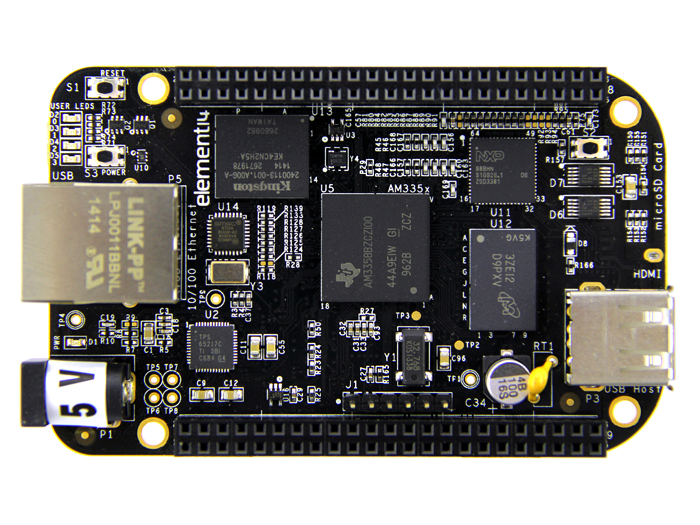
\includegraphics[width=0.4\textwidth]{img/bbb.jpg}
        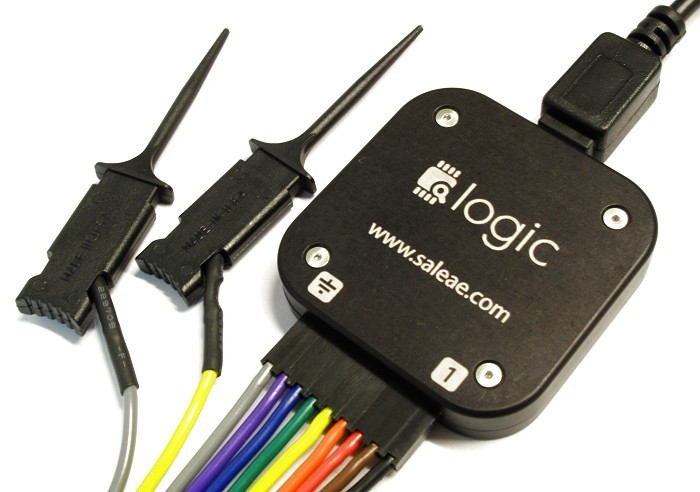
\includegraphics[width=0.3\textwidth]{img/saleae.jpg}
        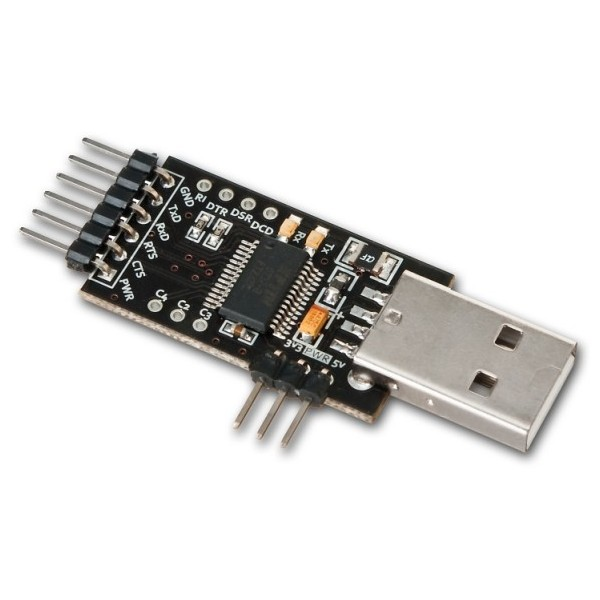
\includegraphics[width=0.28\textwidth]{img/usb.jpg}
        \caption[Devices used in the project]{Devices used in the project: BeagleBone Black\footnote{https://techimperial.in/wp-content/uploads/2017/02/BeagleBone-Black-Rev.C\_02.jpg},
        Saleae Logic 8\footnote{https://www.openlighting.org/wp-content/uploads/2013/12/Saleae-logic.jpg},
        USB$\leftrightarrow$UART\footnote{http://msx-elektronika.pl/pl/wp-content/uploads/2013/10/USB-UART.jpg}.}
    \end{minipage}
\end{figure}


The BeagleBone Black was configured to connect necessary physical pins to PRUs.

Firstly, the input pin of the receiver was connected to the TX pin of the USB-UART interface, so that the receiver can be tested. The Logic analyzer was connected go \textit{spy} on the transmitted signal to verify the correctness of timing. Note that this approach only let the receiver to be tested up to 3MBaud mode, due to the USB-UART limitation.

Then, the input pin of the receiver was connected to the output pin of the transmitter, instead of the USB-UART module, forming a loop. This way, the implemented transmitter module was tested up to 4.168MBaud speed, the maximum. The test was asserted with the Logic analyzer.

\subsection{Possible improvements}

\subsubsection{Timing constraints in the receiver}
Every time 16 bits are read ( 2 bits received ), majority voting is performed. Currently, after optimizations using lookup tables for voting, the voting and saving the result take $46$ cycles. When running at 4.168MBaud, 2 bits are received every $48$ cycles, so there is not much too spare. Perhaps, with further optimizations, a transmitter could be implemented to bit-bang bits while the receiver waits for the next 16-counter event.

\subsubsection{Jitter sensitivity}
Implementing the receiver to work with transmissions of exacly one byte (10 bits due to UART start/stop bits) allows to easily synchronize with every start bit, and therefore sustain a $\pm5\%$ jitter. However, in case of a transmission of consecutive bytes, the receiver may not have time to reset the 16-counter event and ensure synchronization. This introduces sensitivity of $\pm0.006\%$ with transmissions of 64 consecutive bytes (calculation: the receiver may be off by 4 bits maximum to still be able to recover the data). Receiver's code will need to be improved if the user requires higher tolerances for jitter in log messages.

\subsection{Conclusions}

Despite several challenges, such as the lacking documentation of the PRUs, the project was successful.
The critical path in receiver's code only needed 46 clock cycles after optimizations, and at 4.168MBaud transmission, the critical path was executed every 48 clock cycles, which further proofs the hard real-time capabilities of the PRU.

Testing environment chosen turned out to be optimal. Especially helpful was the logic analyzer, with which
the timing of the signals could be easily verified. Perhaps, the debugger could be helpful, but at the point
of writing this report, the usage of the available debugger for the PRU is not straightforward.

\begin{center}
    \label{maximum}
    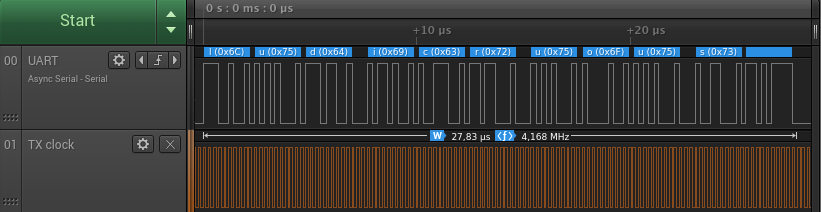
\includegraphics[width=\textwidth]{img/maximum.png}
    \captionof{figure}{Successful transmission at 4.168MBaud}
\end{center}

\subsection{Public code repository}
The developed code is available under MIT license:
\url{https://github.com/phaezah7/UART}.


\bibliographystyle{plain}
\bibliography{report}

% \begin{enumerate}
%     \item \label{compiler} PRU Optimizing C/C++ Compiler - \url{http://www.ti.com/lit/ug/spruhv7b/spruhv7b.pdf}
% \end{enumerate}

\end{document}
